
\chapter{Architecture of Histo}
\label{sec:histo}

Based on the requirements and the evaluation of CouchDB we derive a new architecture for a practical synchronization solution.

\begin{itemize}
\item
  \textbf{No Timestamps}: history-based 3-way merging
\item
  \textbf{No Change Tracing}: explicit change tracing is not necessary - support
  diff computation on the fly
\item
  \textbf{Data Agnostic}: leave diff and merge of the actual data to
  plugins
\item
  \textbf{Distributed}: synchronization does not require a central server
\item
  \textbf{Functional Design}: only implement the functional parts of synchronization - leave everything else to the application (transport, persistence)
\item
  \textbf{Sensitive Defaults}: have defaults that `just work' but
  still support custom logic (e.g. for conflict resolution)
\item
  \textbf{Cross-Platform}: be available on every major platform through the use of Web Standards
\end{itemize}


\section{Hierarchical Data Model Mapping}
\label{sec:histo.hierarchy}
Our data described in the scenario is structured through entity instances, their attribute values and relationships to other instances.
Most modern web application frameworks realize one-to-one relationships, by simply having an attribute storing the related instance's ID.
One-to-many relationships are realized through an attribute having a collection of 
instance IDs as its value.\\
Instance collections often have a relevant order that needs to be preserved.
An example is the list of tasks in a project that is displayed to the user.
The user wants to be able to change the order of tasks and the order should be persisted.\\
We further differentiate between linking to a separately stored instance and  embedding an instance.
An embedded instance can still be linked from other instances but it cannot be embedded twice.
Linking to an instance means to simply hold another instance's ID as an attribute value, embedding means to hold both their ID and actual state.\\

The merge and commit processes, described in the next sections, depend on a hierarchical representation of our application state.
To have a hierarchy we need to define a single root structure, from where all substructures of our state can be reached.\\
Our hierarchical structure can be as simple as this:

\begin{itemize}
\item Level 0 (Root): list of entities
\item Level 1: list of instances per entity
\item Level 2: list of attributes per instance
\end{itemize}

This gives us a very flat tree with each entity node linking to a potentially large number of instances.
For example, our comments entity would directly link to all comments across all projects and tasks.
The next sections will show that it is beneficial for merging performance if each tree node only links to a small number of child nodes.\\
This is where the difference between linking and embedding comes into play.
We can achieve a deeper hierarchy by embedding certain instances in others.
In our scenario we could decide to embed tasks inside projects through one of its attributes.
Comments could in turn be embedded inside tasks.\\
In order to develop a merging algorithm we need to map each substructure of our hierarchy to a suitable data structure.\\
Starting at the top we choose the list of projects as the root structure of our data.
The project list is represented through a \emph{dictionary} embedding all project instances.
The dictionary keys are the instance IDs and the dictionary values embed the actual instances.\\
Each instance is again represented through a \emph{dictionary}.
The dictionary keys correspond to the attributes and the dictionary values to attribute values.\\
If the attribute values are atoms, the hierarchy stops here.
Attributes with string values can be represented with \emph{ordered lists}.
Attribute values linking to other instances are represented through \emph{(ordered) sets}.
We can choose a set as the list can only contain unique instance IDs.\\
Attribute values embedding other instances are represented through an \emph{(ordered) dictionary}.
Like in our project list at the beginning, keys are the IDs of instances and values their actual state.\\
If other instances are embedded, they are kept as children in the hierarchy.\\

Let us summarize the full mapping between model elements and data structures:

\begin{itemize}
\item Instances and their attributes: dictionaries
\item String values: ordered lists
\item Collections linking to instances: (ordered) sets
\item Collections embedding instances: (ordered) dictionaries
\end{itemize}

\begin{figure}[hierarchy]
  \centering
  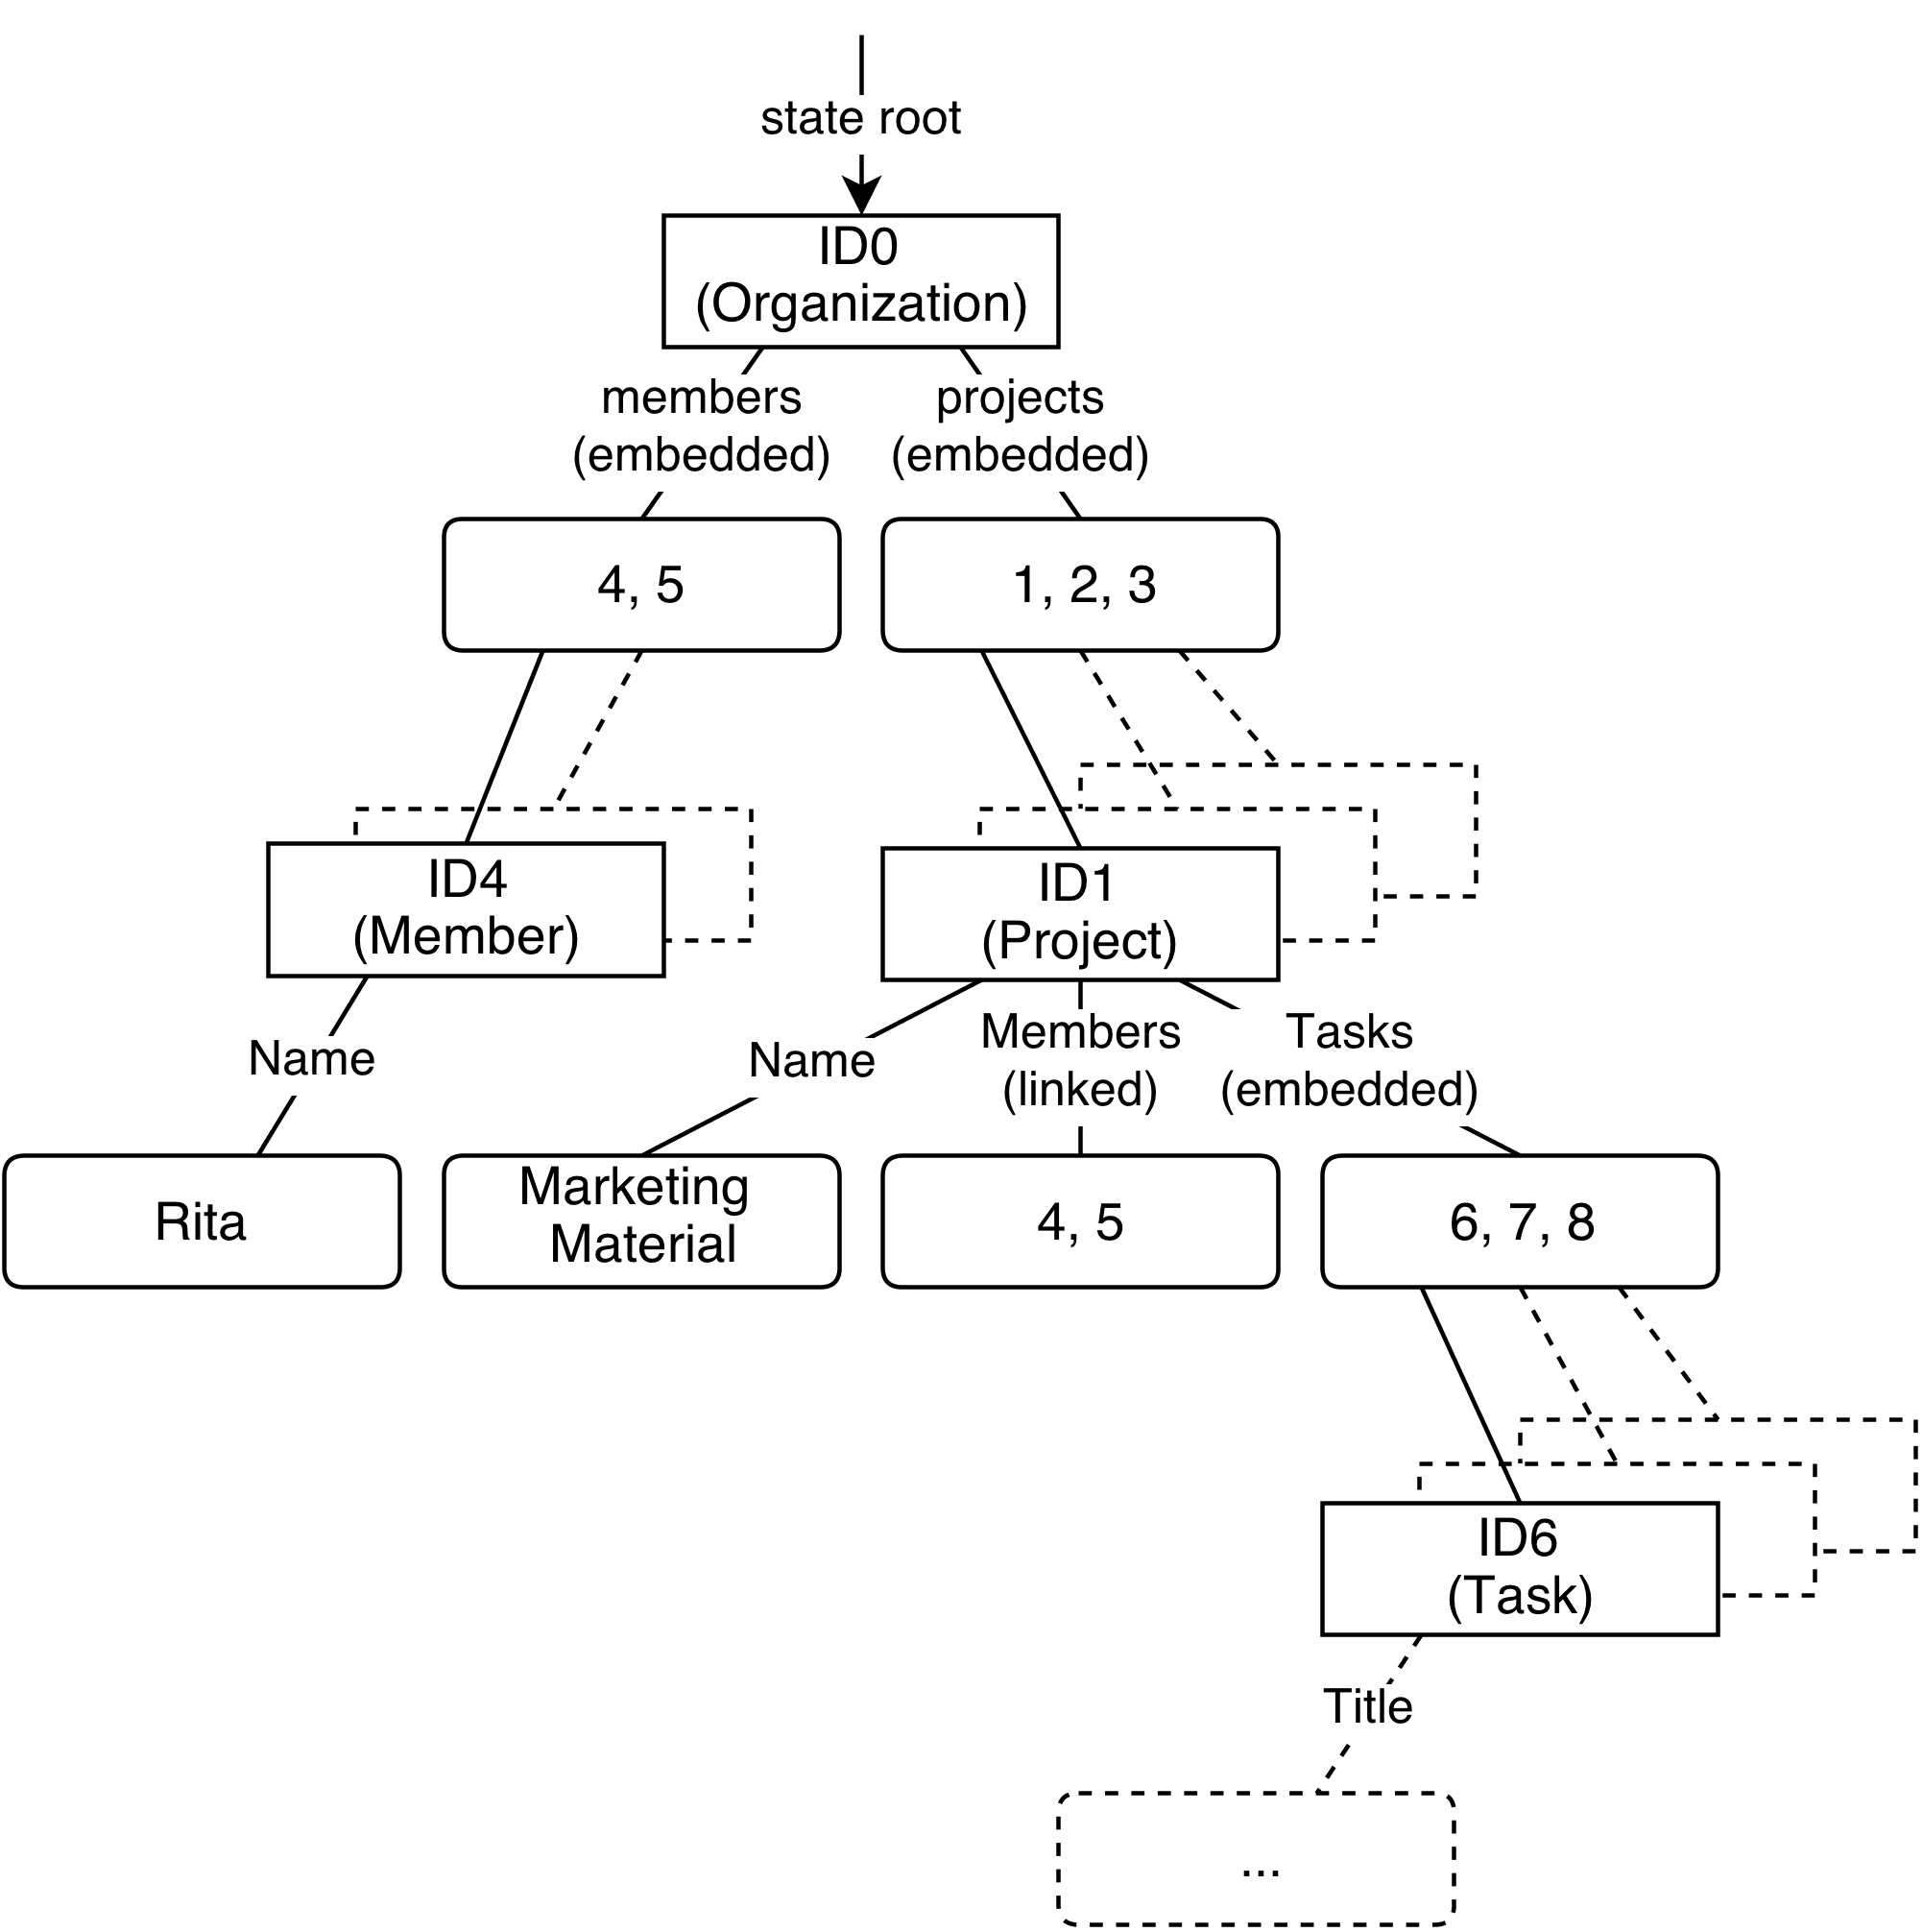
\includegraphics[width=0.8\textwidth]{img/hierarchy}
  \caption{The data model mapped to a hierarchy.}
  \label{fig:histo.hierarchy}
\end{figure}

Figure \ref{fig:histo.hierarchy} shows the actual hierarchy we derived from the data model in our scenario.



\section{Committing Objects}
\label{sec:histo.committing}
We have seen how through the use of object embedding we can structure our data hierarchically.
When persisting our data we do not actually physically embed entire objects down the hierarchy.
If we did this we would end up with a single, big structure which would have to be re-written every time a small change was made.
We therefore store even embedded objects as separate structures.
At a logical level they are still embedded though - we achieve this through the use of cryptographic hashing.
All of our objects are stored in a content-addressable store which is described in Section \ref{sec:background.cas}.
Existing objects are never overwritten - a new version is written instead.
We can retrieve each object based on a cryptographic hash of its content.
When logically embedding an object we actually save it in the store and only reference its hash.\\
Saving each object separately we can now re-use objects of previous states when new data is commited.
As shown in Figure \ref{fig:histo.commits} each data update is represented through a new commit object.
Each commit object points to the root of the data hierarchy and therefore to a snapshot of the entire data.
Commit objects link to their parent commits and are therefore connected in a directed, acyclic graph.\\
Commit objects themselves are stored separately in a content-addressable store.
They reference the root of the data hierarchy through the hash of the root object.
Ancestor commits are simply referenced through their hash as well.\\
Whenever an object in our graph changes, we only need to write the changed object and all its parents again.
All unchanged objects can be referenced again through their state hash.
If we run a commit and no data has actually changed, we therefore do not write any new object versions to the store.\\

Let us go through the steps of an exemplary update which could have lead to the scenario shown in figure \ref{fig:histo.commits}:

\begin{enumerate}
\item A new task with ID10 is added to project ID3 and committed.
\item Task ID10's state is written to the content-addressable store, which returns its cryptographic hash.
\item Project ID3, which embeds Task ID10 references the new hash in its `tasks' attribute, Task ID9 is unchanged and can therefore be referenced without writing it again.\\
The new state of Project ID3 has to be written again returning its new hash.
\item Organization ID0 embeds Project ID3 and therefore has to update the hash in its `projects' attribute to the new version.\\
All other projects and entries of the `members' attribute can reference to the previous instance hashes without writing them again.
\item The new commit object links to the new hash of organization ID0 as the root object.
\item The new commit object links to the previous commit object.
\end{enumerate}

\begin{figure}[commits]
  \centering
  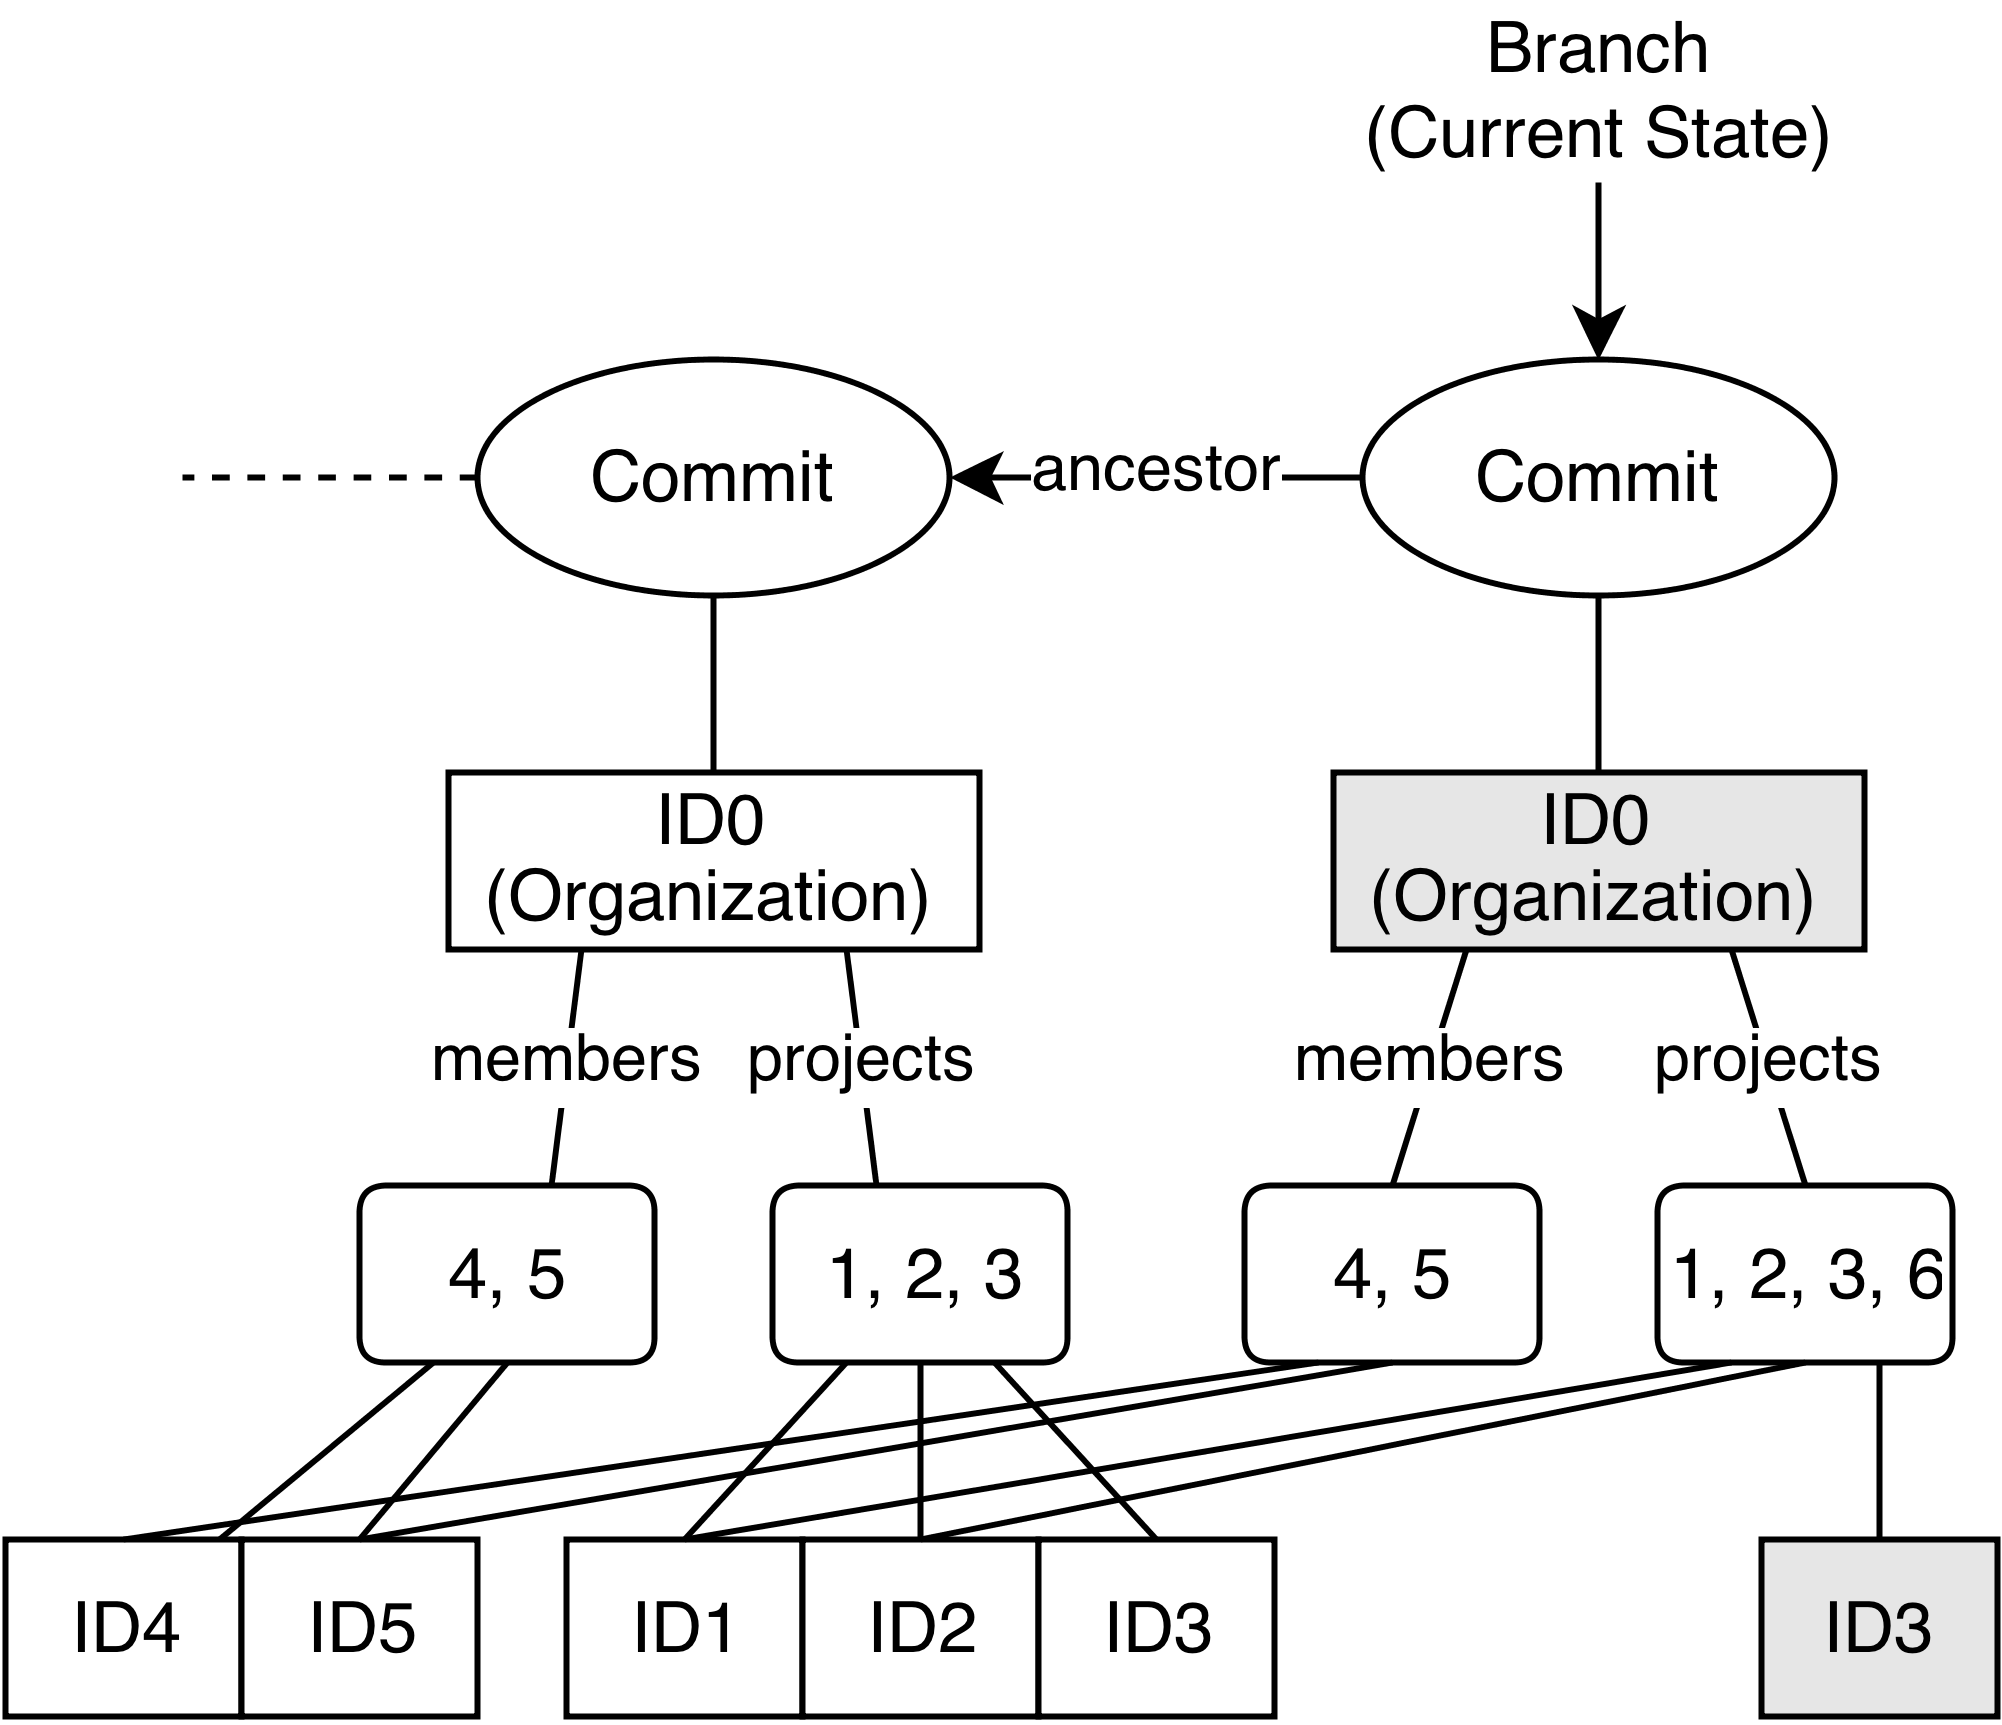
\includegraphics[width=0.6\textwidth]{img/commits}
  \caption{Re-using objects across commits.}
  \label{fig:histo.commits}
\end{figure}

With this model of hierarchical data at hand we can now go into the details of merging two branches of our state.



\section{Synchronization Protocol}
\label{sec:histo.protocol}
Synchronization always happens from a \emph{source} node to a \emph{target} node.
If it is run simultaneously with source and target exchanged, it keeps both nodes in sync with each other.\\
The algorithm is designed to be able to run independently of the source or target.
It could be implemented as a separate application, possibly even running on a different device - as long as it has access to both the source and target node.\\
The synchronizer could be run in regular intervals or explicitly triggered by changes in the source node.
Our solution therefore shares high-level characteristics with CouchDB's solution described in Section \ref{sec:couchdb.protocol}.\\

The latest commit on a node we refer to as its \emph{head}.
A node has a \emph{master head}, which refers to the version of the data considered to be `true' by the node.\\
For each remote node it synchronizes with, the node keeps a \emph{remote tracking head}.\\
A remote tracking head represents what the local node considers to be the current state of a remote node.\\
Before each synchronization, both nodes should commit their latest changes as described in Section \ref{sec:histo.committing}.
Commits snapshot the state of our data as we start synchronizing.
Between synchronizations they do not have to be run on every change of data.
The commit history therefore marks the history of synchronizations between nodes.
Every commit corresponds to the state of one or more synchronizations.

Synchronization follows a two-step protocol, step one propagates all changed data from source to target, step two executes a local merge operation.

\subsection{Update Detection and Propagation}
\label{sec:histo.protocol.detection-propagation}
The combination of update detection and propagation follows the following protocol:

\begin{enumerate}
\item Read the target's remote tracking head of source.
\item Read all commit IDs since the target's remote tracking head from source and write them to target.
\item Let the target compute the common ancestor commit ID of target's and source's master heads.
\item Read all changed data since the common ancestor commit from source and write to target.
\item Set the target's remote tracking head of source to source's master head.
\end{enumerate}

Once these steps are executed, the target node has the current state of source available locally.\\
The target's head still refers to the same state as the source data has not been merged.\\

Listing \ref{propagation-protocol} summarizes the protocol as pseudo-code.\\

\begin{lstlisting}[caption=Detecting updates across nodes and propagating the changes., label=propagation-protocol]

sourceHead = source.head.master
targetHead = target.head.master
lastSyncedCommit = target.getRemoteTrackingHead(source.id)

commitIDssource = source.getCommitDifference(lastSyncedCommit, sourceHead)

target.writeCommitIDs(commitIDssource)

commonAncestor = target.getCommonAncestor(targetHead, sourceHead)

changedData = source.getDataDifference(commonAncestor, sourceHead)

target.writeData(changedData)

target.setRemoteTrackingHead(source.id, sourceHead)

\end{lstlisting}

The functions `getCommitDifference()' and `getDataDifference()' are implemented as described in Section \ref{sec:histo.diff-across-commits}.\\
The most recent common ancestor algorithm used in `getCommonAncestor()' is described in Section \ref{sec:background.lca}.\\
The internals used by `writeData()' and the underlying commit data model have been explained in Section \ref{sec:histo.committing}.\\
Note that keeping the remote tracking head is optional.
The protocol still succeeds if the remote head is unknown or rembered wrong.
Section \ref{sec:histo.topologies.multi-master} will illustrate this for a multi-master topology. 

\subsubsection*{Robustness}
The data propagation protocol can fail at any point without leaving either node in an inconsistent state.
The phase does not override any data on the nodes besides the remote tracking head on the target.
If the protocol fails before updating the remote tracking head, it simply has to be repeated.

\subsection{Merging}
\label{sec:histo.protocol.merging}
Even if the source is disconnected at the merging stage, the target has all the necessary information to process the merge offline.\\

The target's master head we refer to as the \emph{master head}.
The target's remote tracking branch for the source we refer to as the \emph{source tracking head}.
From a high-level the algorithm can be described as the following:\\

\begin{enumerate}
\item Compute the common ancestor of the master head and the source tracking head. (The common ancestor could also be re-used from the propagation step.)
\item If the common ancestor equals the source tracking head:\\
  The source has not changed since the last synchronization. The master head is ahead of the source tracking head.\\
  The algorithm can stop here.
\item If the common ancestor equals the master head:\\
  The target has not changed since the last synchronization.\\
  The source's head is ahead of target.\\
  We can fast-forward the master head to the source tracking head.
\item If the common ancestor is neither the source tracking head nor the master head:\\
  Both source and target must have changed data since the last synchronization.\\
  We run a three-way merge of the common ancestor, source tracking head and master head.\\
  We commit the result as the new master head.
\end{enumerate}

This protocol is able to minimize the amount of data sent between synchronized
nodes even in a distributed, peer-to-peer setting.
Section \ref{sec:histo.topologies} will look at the protocol's support of various network topologies.\\

Updating the target's head uses optimistic locking.
To update the head you need to include the last read head in your request.
So both the fast-forward operation or the commit of a merge result can be rejected if the target has been updated in the meantime.
If this happens the Synchronizer simply has to re-run the merge algorithm.\\

In Figure \ref{fig:histo.merging-protocol}, the merging process is described using pseudo-code.\\
Its core is the call to `three-way-merge()' - the details of our three-way merging concepts are described in Section \ref{sec:histo.merging}.\\

\begin{lstlisting}[caption=Merging Protocol, label=fig:histo.merging-protocol]

masterHead = target.head.master
sourceTrackingHead = target.head.sourceID

commonAncestor = target.getCommonAncestor(masterHead, sourceTrackingHead)

if (commonAncestor == sourceTrackingHead) {
  // do nothing

} else if (commonAncestor == masterHead) {
  // fast-forward master head
  try {
    // when updating the head we have to pass in the previous head:
    target.setHead(sourceTrackingHead, masterHead)
  } catch {
    // the master head has been updated in the meantime
    // start over
  }

} else {
  commonAncestorData = target.getData(commonAncestor)
  sourceHeadData = target.getData(sourceTrackingHead)
  targetHeadData = target.getData(masterHead)

  mergedData = three-way-merge(commonAncestorData, sourceHeadData, targetHeadData)

  // commit object linking commit data with its ancestors:
  commitObject = createCommit(mergedData, [masterHead, sourceTrackingHead])

  try {
    // when updating the head we have to pass in the previous head:
    target.commit(commitObject, masterHead)    
  } catch {
    // the master head has been updated in the meantime
    // start over
  }
}

\end{lstlisting}

The protocol described here only propagates the changes from the source to the target node.
To actually synchronize both nodes to the same state, the protocol has to be run in the reverse direction as well.

\subsubsection*{Robustness}
Running the protocol in both directions is not an atomic operation.
It is therefore possible that both nodes do not end up with the exact same state as updates to the data can be made on both nodes at any time.
The nodes are only consistent if both nodes do not change any data while the synchronization takes place.
This is actually part of our requirements of supporting optimistic synchronization and to only guarantee eventual consistency, which are defined in Section \ref{sec:requirements.optimistic}.\\
The merging protocol is unlikely to fail as it runs entirely on the local node without requiring error-prone network communication.
In case of the fast-forward merge, only the local head is updated to the source tracking head.
This operation can fail if the local head was updated in the meantime.
The merge protocol then simply has to be repeated.\\
A failure in the three-way-merge call (line 25) does not corrupt any data, as the local head remains unchanged.
Only after a successful merge, a new commit object is created and the local head is updated.
Again, there can be a failure if the local head has been updated while the merge operation is running.
In this case the merge protocol is repeated as well to include the latest changes in the merge.
Note that in any case of failure, only the merge protcol has to be repeated but not the comparatively long-running data propagation protocol.



\section{Update Detection Between Branches}
\label{sec:histo.diff-across-commits}

The change detection phase of our synchronization protocol is defined through the calls `getCommitDifference()' and `getDataDifference()'.
We will now look into the internals of the algorithms invoked through these calls.\\

\subsection{Commit History Difference}
Identifying added commit IDs since a last known synchronized commit is only working on the meta-data level - there is no application data involved in this phase.\\
Given two branches A and B we want to retrieve all commits A needs in order to be in sync with B.
Our algorithm is based on the recursive invocation of a lowest common ancestor implementation:\\

\begin{enumerate}
\item Compute the lowest common ancestor of commit A and B.
\item Add commit B to the result.
\item Walk up the ancestor chain of commit B, adding all commits to the result unless:
\item The common ancestor is reached - then return the result.
\item If a commit has multiple ancestors - then invoke the algorithm again with each ancestor as commit B.\\
Add the result of the recursive invocation to the final result.
\end{enumerate}

We can express this more concretely using pseudo-code:\\

\begin{lstlisting}[caption=Detecting commit history difference, label=commit-difference]

function getCommitDifference(commitA, commitB) {
  result = []

  commonAncestor = getCommonAncestor(commitA, commitB)

  while (not commitB.hasMultipleAncestors()) {
    singleAncestor = commitB.getAncestors()[0]

    if (singleAncestor == commonAncestor) {
      return result
    }

    result.push(singleAncestor)

    commitB = singleAncestor
  }

  ancestors = commitB.getAncestors()

  for (each ancestor in ancestors) {
    forkResult = getCommitDifference(commitA, commitB)
    result.append(forkResult)
  }

  return result
}

\end{lstlisting}

Figure \ref{fig:histo.new-commits} visualizes the commit difference for two branches B and C.
The last synchronized commit is A.
B has in the meantime made concurrent changes and it has synchronized with another branch D.
Branch D has not been synchronized with branch C.
The commit difference between A and B is therefore the sum of two commit paths:\\

\begin{itemize}
\item The shortest commit path between B and the lowest common ancestor of A and B, which is B.
\item The shortest commit path between D and the lowest common ancestor of D and A, which is E.
\end{itemize}

\begin{figure}[new-commits]
  \centering
  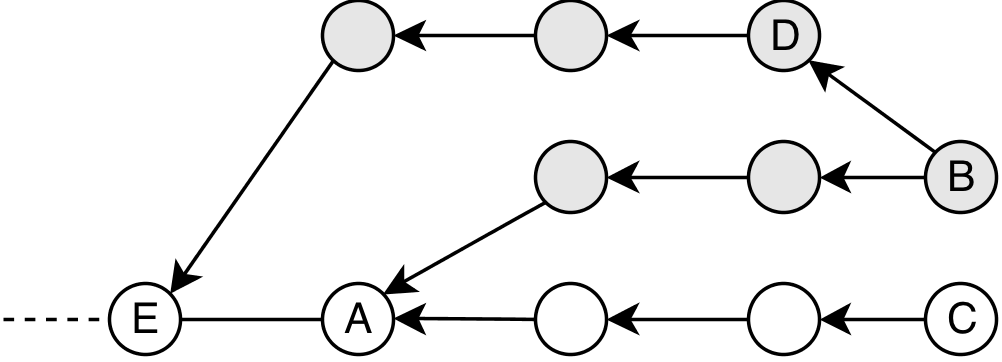
\includegraphics[width=0.6\textwidth]{img/new-commits}
  \caption{Commit difference between branches B and C and A being the last synchronized commit.}
  \label{fig:histo.new-commits}
\end{figure}

\subsection{Application Data Change Detection}

Having extracted the list of commits that need to be propagated we can now trace what data has been changed through these.\\
In section \ref{sec:histo.committing} we explained how each object is stored separately under its cryptographic hash.
Existing objects are never updated in-place - we therefore only have to identify which objects have been added to the store.\\

We identify updated objects on a per-commit basis comparing each commit's state with its ancestors.
Starting at the root object referenced by the commit we recursively difference the hierarchy with the commit's ancestor:

\begin{lstlisting}[caption=Detecting data difference across commits, label=data-difference]

function getDataDifference(rootObjectHash, ancestorRootObjectHash) {
  result = []

  if (rootObjectHash == ancestorRootObjectHash) {
    return result
  }

  result.push(rootObjectHash)

  rootObject = store.read(rootObjectHash)
  ancestorRootObject = store.read(ancestorRootObjectHash)
  rootChildren = rootObject.getChildDictionary()
  ancestorChildren = ancestorRootObject.getChildDictionary()

  childDifference = getDictionaryDifference(ancestorChildren, rootChildren)

  for (each insertedChildHash in childDifference.inserts) {
    insertedChildAllChildren = getChildrenRecursive(insertedChildHash)
    result.push(insertedChildHash)
    result.concat(insertedChildsAllChildren)
  }

  for (each update in childDifference.updates) {
    updatedChildHash = update.new
    updatedAncestorChildHash = update.ancestor
    childResult = getDataDifference(updatedChildHash, updatedAncestorChildHash)
    result.concat(childResult)
  }

  return result
}

\end{lstlisting}

In our scenario the children correspond to embedded instances as we defined them in section \ref{sec:histo.hierarchy}.
While in our data model we differentiate between instances belonging to certain attributes this is not relevant for the data difference algorithm.
We simply flatten the embedded child instances across all attributes to a single dictionary of children.\\
The dictionary difference algorithm that is used in the `getDictionaryDifference()' call is explained in section \ref{sec:histo.merging.diff}.
In the context of the section it is used for merging but we can re-use the algorithm for our purpose here.\\
Through the combination of the commit and data difference algorithms we now have the tools to implement the update detection and update propagation steps of our synchronization protocol as described in section \ref{sec:histo.protocol}.



\section{Reconciliation Through Three-Way Merging}
\label{sec:histo.merging}
In this section we will focus on three-way merging which is part of the reconciliation phase of our protocol developed in section \ref{sec:histo.protocol.detection-propagation}.\\
All necessary data for a merge has already been propagated from the source to the target node.
We have all information about the current state and the commit history of the source node available locally.
The current state is marked through the source tracking branch as described in section \ref{sec:histo.protocol.merging}.
The entire merging process can therefore happen offline without the need of any communication with the source node.\\
Our three-way merge algorithm is structured into three types of processes which are recursively executed on our data hierarchy:

\begin{itemize}
\item \textbf{Differencing}: we diff branch B and C with their common ancestor A.
\item \textbf{Merging}: we merge the two diffs A-B and A-C to a new diff result.
\item \textbf{Patching}: we apply the merged diffs as a patch to A which results in the merged state D.
\end{itemize}

Our current branch we refer to as B and the source tracking branch as C.
The common ancestor of B and C is defined as A.\\
Starting with a differencing phase we identify the changes made in the branches B and C since our common ancestor state A.\\
If follows a diff merging phase where the two diff results A-B and A-C are combined into one diff.
As its only input is the two diffs it does not require access to the actual states A, B or C.
In this phase conflicts can appearch if the two branches contain updates to the same parts of the state.\\
The merged diff can then be applied to the origin state A in order to create the actual merged state.
For this step we require a patch algorithm.\\
These three steps are actually applied to each hierarchy level or our state.
In the next section we give concrete examples of what the expected output of each level should be.
Based on the examples we will then look into implementation details of the respective algorithms.

\subsection{Merge Scenario}
\label{sec:histo.merging.scenario}
To show correctness of a merge algorithm we need to define sample model states with expected merge results.
This set of data can then be used as a test case for our implementation.
Based on an ancestor state all users start with, we define several possible branch states.\\
Merging of the branch states will happen at multiple levels of detail corresponding to our data hierarchy.
Each level will have its own difference and diff merge phase.
The result of the diff merge phases is then used to patch the common ancestor state.\\
The difference and merge algorithms that need to be applied will vary on each level depending on the data structures used.
The sample data is defined so that we can demonstrate each possible data structure that we mapped to in section \ref{sec:histo.hierarchy} (dictionaries, ordered dictionaries, ordered sets and ordered lists).\\

The root of our state is defined through an organization instance.
All other instances can be reached from it.
As defined in section \ref{sec:histo.hierarchy}, we differentiate between linking and embedding of instances.
Linking is done by only referencing an instance's ID, embedding is done by referencing its actual state hash along with the ID.\\

\begin{tabularx}{0.8\textwidth}{ l l X X }
\multicolumn{4}{ c }{\textbf{Ancestor state A of Organization}} \\
ID & Hash & Members (embedded) & Projects (embedded) \\
\hline
0
& O0A
& 1: U1A \newline 2: U2A \newline 3: U3A
& 4: P4A \newline 5: P5A \newline 6: P6A \newline 7: P7A
\end{tabularx} \\
\\

For completeness we include the state of embedded user instances - they will not be modified in this example:\\

\begin{tabularx}{0.3\textwidth}{ l l l }
\multicolumn{3}{ c }{\textbf{Ancestor state A of Users}} \\
ID & Hash & Name \\
\hline
1 & U1A & Rita \\
2 & U2A & Tom \\
3 & U3A & Allen
\end{tabularx} \\
\\

The projects embedded in the organization show the difference between linking (members) and embedding (projects):\\

\begin{tabularx}{\textwidth}{ l l l l X }
\multicolumn{5}{ c }{\textbf{Ancestor state A of Projects}} \\
ID & Hash & Project Name & Members (linked) & Tasks (embedded, ordered) \\
\hline
4 & P1A & Marketng Material & 1, 2, 3
& 8: T8A \newline 9: T9A \newline 10: T9A \newline 11: T11A
\\
5 & P5A & Product Roadmap & 1, 3 & 12: T12A
\\
6 & P6A & Staffing & 1 & 13: T13A \newline 14: T14A
\\
7 & P7A & Finances & 3 & 15: T15A
\end{tabularx} \\

We will leave out the details on the state of other entities (tasks and comments) as the instances shown so far already cover all required modeling aspects.\\

The state has been modified resulting in a new state in branch B:\\

\begin{tabularx}{0.8\textwidth}{ l l X X }
\multicolumn{4}{ c }{\textbf{State B of Organization}} \\
ID & Hash & Members (embedded) & Projects (embedded) \\
\hline
0
& O0AB
& 1: U1A \newline 2: U2A \newline 3: U3A
& 4: P4A \newline 5: P5A \newline 6: P6A \newline 7: P7A
\end{tabularx} \\
\\

\begin{tabularx}{\textwidth}{ l l l l X }
\multicolumn{5}{ c }{\textbf{State B of Projects}} \\
ID & Hash & Project Name & Members (linked) & Tasks (embedded, ordered) \\
\hline
4 & P1AB & Marketing Material & 1, 2
&
8: T8A \newline
11: T11A \newline
9: T9A \newline
10: T9A \newline
17: T17B
\\
5 & P5AB & Product Roadmap & 1, 3 & 12: T12A
\\
6 & P6A & Staffing & 1 & 13: T13A \newline 14: T14A
\\
7 & P7A & Finances & 3 & 15: T15A \newline 18: T18B
\\
16 & P16B & Sales Planning & 1, 2 & 
\end{tabularx} \\
\\

Through concurrent updates branch C emerged - its state is defined as the following:\\

\begin{tabularx}{0.8\textwidth}{ l l X X }
\multicolumn{4}{ c }{\textbf{Ancestor state C of Organization}} \\
ID & Hash & Members (embedded) & Projects (embedded) \\
\hline
0
& O0AC
& 1: U1A \newline 2: U2A \newline 3: U3A
& 4: P4AC \newline 5: P5AC
\end{tabularx} \\
\\

\begin{tabularx}{\textwidth}{ l l l l X }
\multicolumn{5}{ c }{\textbf{State C of Projects}} \\
ID & Hash & Project Name & Members (linked) & Tasks (embedded, ordered) \\
\hline
4 & P1AC & Marketing Strategy & 1, 2, 3
& 11: T11A \newline 8: T8A \newline 9: T9A \newline 10: T9A
\\
5 & P5AC & Product Strategy & 1, 3 & 12: T12A \newline 19: T19C
\end{tabularx} \\

We start the merging process with the root instance hashs:\\

\begin{tabular}{ l l l l l }
\multicolumn{5}{ c }{\textbf{Organization difference}} \\
ID & State A & State B & State C & Result \\
\hline
0 & O0A & O0AB & O0AC & conflict (concurrent update)
\end{tabular} \\

Both B and C have obviously modified the content of our organization in different ways resulting in a conflict.\\
We will try to resolve this conflict by differencing the data on a more detailed level.
The value of the `members' attribute has not been modified - we therefore look at the difference of the `projects' attribute: \\

\begin{tabular}{ l l l l l }
\multicolumn{5}{ c }{\textbf{`Projects' attribute difference of organization ID 0}} \\
ID & State A & State B & State C & Result \\
\hline
4 & P4A & P4AB & P4AC & conflict (concurrent update) \\
5 & P5A & P5AB & P5AC & conflict (concurrent update) \\
6 & P6A & P6A & - & remove \\
7 & P7A & P7AB & - & conflict (concurrent update and remove) \\
16 & - & P16B & - & insert
\end{tabular} \\
\\

Whenever the hash of an instance has only changed in one state, we carry the change over into the result.
If the hash has changed in both states, we have a conflict.
This merging phase will be implemented through difference and merge algorithms for dictionaries.\\
We will try to resolve conflicts by running a finer grained merge on the conflicting instance states.
ID 4 and ID 5 will therefore go into a lower level of merging while the changes in ID 6 and 16 are already accepted.
We cannot run a finer grained merge on ID 7 as it was removed in state C.
This conflict can therefore not be resolved and directly carried into the result.\\

Lets see if we can resolve conflicts 4 and 5 in the next merge.
At this level we will again look at individual attributes to find out which are actually affected by the updates.\\

\begin{tabularx}{\textwidth}{ l X X X l }
\multicolumn{5}{ c }{\textbf{Attribute difference of task ID 4}} \\
Attribute & State A Hash & State B Hash & State C Hash & Result \\
\hline
Project Name & Markting Material & Marketing Material & Marketing Strategy & conflict \\
Members & 1, 2, 3 & 1, 2 & 1, 2, 3 & update
\\
Tasks &
8: T8A \newline 9: T9A \newline 10: T9A \newline 11: T11A
&
8: T8A \newline
11: T11A \newline
9: T9A \newline
10: T9A \newline
17: T17B
& 11: T11A \newline 8: T8A \newline 9: T9A \newline 10: T9A
& conflict
\end{tabularx}\\
\\

At this level we can already carry over the update of the `Members' attribute in B to the result.\\
The `Project Name' and `Tasks' attributes of B and C have been concurrently updated and are therefore in conflict.
This difference and merge step can again be realized with an algorithm for dictionaries (keys being attributes, values being attribute values).\\
If we define string values as atoms we have reached the most detailed level of merging for `Project Name' - the conflict will therefore be carried over into the result.
If we instead see strings as another substructure we can attempt to resolve the conflict by using a string merging algorithm.\\
We have mapped the embedded and ordered `Tasks' attribute to an ordered dictionary data structure.
We can therefore try to resolve the conflict by applying a merge algorithm for ordered dictionaries.\\

We will now describe the result we expect from merging the `Project Name' strings.
Note that all index positions in the following diffs are seen as relative to the ancestor state.
So even if one diff contains multiple insert or remove operations they are given as if they were all applied simultaneously to the ancestor state.\\

\begin{tabularx}{\textwidth}{ l X X }
\multicolumn{3}{ c }{\textbf{`Project Name' difference for project ID 4}} \\
Diff A-B & Diff A-C & Diffs Merged \\
\hline
insert `i' behind index 5 & insert `i' behind index 5 \newline remove from index 9 to 17 & insert `i' behind index 5 \newline remove from index 9 to 17
\end{tabularx}\\
\\

Applying this merge result to the ancestor state gives us an intuitive result: `Marketing Strategy'.\\

To merge the ordered dictionary structure representing the `Tasks' attribute we will apply two separate merge steps:

\begin{itemize}
\item Order merge: We can merge the order by using the keys of the ordered dictionary as an ordered set and applying an ordered set merge algorithm.
\item Value merge: The values are merged by applying an ordinary dictionary merge algorithm. 
\end{itemize}

The expected output of the order merge for the `Tasks' attribute:\\

\begin{tabularx}{\textwidth}{ X X X }
\multicolumn{3}{ c }{\textbf{`Tasks' order difference for project ID 4}} \\
Diff A-B & Diff A-C & Diffs Merged \\
\hline
move index 3 behind index 0 \newline insert 6 behind index 3
& move index 3 behind index -1
& insert 6 behind index 3 \newline
conflict (`move index 3 behind index 0' and `move index 3 behind index -1')
\end{tabularx}\\
\\

We have been able to carry over one operation into the result while we still have an update conflict.
There is no way we can do an even finer grained merge to resolve this conflict.
The application developer will have to implement a custom merge solution - possibly even asking the user which operation to choose.\\
Depending on how the conflict is resolved, possible results are:

\begin{itemize}
\item 8, 11, 9, 10, 17
\item 11, 8, 9, 10, 17
\end{itemize}

The value merge works analog to the merge we did for the `Projects' attribute in the organization instance.
We will skip this phase as none of the tasks have been updated.\\

The merge of ID 5 works analogous - we will therefore skip the attribute merging step and jump right into the string merge:\\

\begin{tabularx}{\textwidth}{ X X X }
\multicolumn{3}{ c }{\textbf{`Project Name' difference of project ID 5}} \\
Diff A-B & Diff A-C & Diffs Merged \\
\hline
remove from index 8 to 15 \newline insert `Planning' behind index 7
& remove from index 8 to 15 \newline insert `Strategy' behind index 7
& remove from index 8 to 15 \newline insert `Planning' behind index 7
\newline insert `Strategy' behind index 7
\end{tabularx}\\
\\

We have applied the same merge logic that helped us resolve the name conflict in project ID 4.
But the result we get here is not what a user would expect.
Applying the merged operations to the ancestor state results in: `Product StrategyPlanning'.\\
This is a good example for the violation of intention preservation.
Both in state B and C the user actually intended to \emph{replace} the word `Roadmap'.
Concurrently replacing the same word should clearly cause a conflict.
Our differencing algorithm has no notion of a `replace' operation.
All it sees is a remove of `Roadmap' and an insert of some other word.\\
This example shoes the limits of generic merging algorithms that preserve user intention.\\
In practice it would propably be more suitable to define the `Project Name' as an atom.
As names are short it is more likely that an update is actually intended as a replace operation of the entire string.

\subsection{Differencing}
\label{sec:histo.merging.diff}
Differencing algorithms have been studied extensively.
There exist efficient solutions for a range of data structures.
It is not a focus of our thesis to develop the most efficient differencing algorithm matching our scenario.
Our goal in this section is to show the practical feasibility of the three-way merging component in our architecture.
We favor a simple solution, re-using existing concepts so that we can broaden our focus on an other areas of our synchronization solution.\\
The test case defined in the previous section can be decomposed and mapped to common data structures.\\
The first merging level of instances represented as cryptographic hash can be mapped to a \emph{dictionary} with key-value entries.\\
Same is true for instance-level merging: the dictionary keys are mapped to the attribute names and the dictionary values to the respective value hashs.\\
Attribute values that represent collections of instance IDs can be mapped to \emph{sets}.
Our `Members' attribute does not have a relevant order, it can be mapped to an ordinary set.
The `Tasks' attribute has a significant order and therefore has to be mapped to an \emph{ordered set}.\\
If we do not treat string values as atoms we have to represent them as an \emph{ordered list}.\\

To summarize - for the following data structures we need an algorithm that finds the difference from an origin state A to a changed state B:

\begin{itemize}
\item \textbf{Dictionaries}: to model entity instances and instance attributes.
\item \textbf{Sets and Ordered Sets}: to model instance relationships.
\item \textbf{Ordered Lists / Strings}: to model string values of instance attributes.
\end{itemize}

Ordered list or string data structures have been the main focus in previous research on difference algorithms.
Myers presented an efficient algorithm with $\mathcal O(n*d) $ time and space complexity to difference two strings A and B with
$ n $ representing the sum of the lengths of two strings and $ d $ the size of the shortest edit script transforming A to B \cite{Myers:1986wi}.
The shortest edit script is equivalent to the result of a differencing algorithm.
As in practical applications differences are usually small the algorithm performs well.\\

Given the ordered list difference algorithm we can re-use it to build an algorithm for ordered sets.
Ordered lists can only have differences in the form of \emph{insert} or \emph{remove} operations.
Ordered sets extend this - the simultaneous remove and insert of a globally unique element is now considered as a move operation.\\
To implement an ordered set algorithm we can therefore take the output of the ordered list algorithm and scan the result for the remove and insert of the same element.
This can be efficiently implemented through a hash:

\begin{enumerate}
\item Scan the diff result and build a hash for all removed elements.
\item Scan the result again and test for all inserted elements whether they are included in the hash.
\item If a match is found replace the remove and insert operations through a single move operation in the result.
\end{enumerate}

The time complexity of building a hash can be estimated with $ \mathcal O(n * log(n)) $ with $ n $ representing set size.
The match searching has linear time complexity.
We therefore only add $ \mathcal O(n * log(n)) $ complexity to Myers difference algorithm for a naive solution for ordered sets.\\

For ordinary sets we can implement a simple solution through two hashs of the respective set entries combined with a scan through each set:

\begin{enumerate}
\item Add all entries of set A to a hash $ H_A $ and those of set B to a different hash $ H_B $.
\item Scan set A and test for matches in hash $ H_B $.
\item If no match is found add a remove operation to the result.
\item Scan set B and test for matches in hash $ H_A $.
\item If no match is found add an insert operation to the result.
\end{enumerate}

\emph{Insert} and \emph{remove} are the only operations in a set.\\
The time complexity for building each hash is again $ \mathcal O(n * log(n)) $.
Searching for matches has linear complexity which results in a time complexity $ \mathcal O(n * log(n)) $ for the entire algorithm.\\

A dictionary data structure has \emph{insert}, \emph{remove} and \emph{update} operations.
If the instance described through the dictionary has a fixed set of attributes it would actually only need to support an update operation.
In modern web applications it is not uncommon that there is no fixed data schema.
It is often the case that new attributes are added to instances at runtime.
Even if there is a fixed schema it might be changed through a software update with old instances not being migrated to the new schema.
We should therefore support the full set of dictionary operations in our difference algorithm.

A simple and efficient solution is to again use two hashes for fast lookup combined with a scan through both dictionaries:

\begin{enumerate}
\item All all keys and values of dictionary A to hash $ H_A $ and those of dictionary B to hash $ H_B $.
\item Scan through all key-value entries of A.
\item If the key is not included in hash $ H_B $, add a remove operation to the result.
\item If the key is included and the value in $ H_B $ is different, add an update operation.
\item Scan through all key-value entries of B.
\item If the key is not included in hash $ H_A $, add an insert operation to the result.
\end{enumerate}

Building the hash is again estimated with time complexity $ \mathcal O(n * log(n)) $, scanning both dictionaries has linear time complexity. The combined time complexity is therefore again $ \mathcal O(n * log(n)) $.\\
Depending on the application, its instances are often already implemented with hash-like lookup performance - in this case we could skip step 1.
The time complexity is in this case only linear.\\

\subsection{Diff Merging}
\label{sec:histo.merging.merge}

We will now look into strategies for merging the diff results of the algorithms described in the previous section.
Our focus lies on the identification of potential conflicts based on three-way merging semantics.\\

\emph{Ordered lists} only support insert and remove operations.
Concurrent insert or remove operations are never conflicting as they do not update existing structures.
As we have seen in the example at the end of section \ref{sec:histo.merging.scenario} this is not necessarily in line with a user's intentions.
When editing text users often intend to \emph{replace} content although their actions are represented through a remove and insert operation.
This is why most concurrent version control systems have the notion of \emph{areas} in text.
Concurrent insert or remove operations in overlapping areas are considered as update operations to the same content and therefore result in conflicts.\\
The optimal definition of an area can vary depending on the application.
It may be the entire edited paragraph, a number of lines, sentences, words or even characters.\\
When modeled as an ordered list we can only vary the number of list elements defining the size of an area.\\
Concurrent insert or remove operations which are not in overlapping areas are simply both carried over to the merge result.\\

\emph{Ordinary sets} have the same operations as ordered lists except that each element is unique and we now have no element order.
Without a specified order we can not define \emph{areas}.
Merging two diffs is therefore trivial as no conflicts can occur.
We simply combine the set of operations of both diffs into one large diff.\\

\emph{Ordered sets} add move operations as we can uniquely identify each element.
Move operations can lead to conflicts if the same element is concurrently moved to different locations.
If move operations are not conflicting they are carried over into the merge result.
Insert and remove operations are merged the same way as defined for ordered lists.\\

\emph{Ordinary Dictionaries} have insert, remove and update operations.
Concurrent insert and remove operations never lead to conflicts - they are carried over into the merge result.
Update operations can lead to conflicts if the value of the same key is concurrently modified.

\subsection{Patching}
\label{sec:histo.merging.patching}

Patching is defined as an algorithm applying the identified differences between state A and B as operations to state A.
A computed diff A-B patched to A will result in B.
For our three-way merging algorithm, patching constitutes the last phase. 
Two merged diffs are applied as a patch to the common ancestor state resulting in the actual merged state.\\
We again need patching algorithms for each data structure we intend to support.
The implementation needs to consider that simply executing the operations defined in the diff can lead to a wrong result.
This is true if a change operation has side effects on other parts of the state.\\
In our set of data structures this is only the case for ordered lists and ordered sets.
Applying an insert operation at the specified index, renders the indexes of following operations wrong.
A simple example:

\begin{itemize}
\item State A: `Marketng Matrial'
\item Diff:\\
insert `i' behind index 5\\
insert `e' behind index 11
\end{itemize}

Applying the first diff operation to A results in: `Marketing Matrial'.\\
If we now execute the second operation at the specified index 11 we get: `Marketing Maetrial'.\\
The implementation therefore needs to treat the given indexes as relative positions in the ancestor state.\\
The diff operations of sets and dictionaries can be executed as they are without taking side-effects into consideration.

\subsection{Hierarchical Merging}
As we have seen in our scenario, merging of our structured data is actually a hierachical process combining all of the described algorithms.
Our strategy is to start at the highest-level representing sub-structures using their cryptographic hash.
Whenever we identify an update on the hash of a sub-structure we do a finer grained diff and merge on the structure itself:

\begin{enumerate}
\item Represent all instances of an entity as a dictionary with instance IDs as keys and a cryptographic hash of their attribute values as dictionary values.
\item Use the dictionary diff algorithm to identify inserted, removed and updated instances on A-B and A-C.
\item Merge the dictionary diffs to result \emph{M1}.
\item Remove each instance with an update conflict from \emph{M1}.\\
Represent it as a dictionary with keys being attribute names and values being a cryptographic hash of attribute values.
\item Use the dictionary diff algorithm to identify inserted, removed and updated attributes.
\item Merge the per-instance diffs to result \emph{M2}.
\item Remove each non-atomic attribute with an update conflict from \emph{M3}.\\
Run the respective algorithm:\\
Attributes with (ordered) sets of instance IDs: (ordered) set diff algorithm.\\
Attributes with string values: ordered list diff algorithm.
\item Merge the attribute diffs to result \emph{M3}.
\item Resolve all remaining conflicts in \emph{M1}, \emph{M2} and \emph{M3} manually.
\item Patch the respective substructures of state A using \emph{M1}, \emph{M2} and \emph{M3}.
\end{enumerate}

This approach can not only be applied to difference entity-relationship models, it can actually be adapted for any type of data with a hierarchical structure.



\section{Handling Conflicts}
\label{sec:histo.conflicts}

Conflicts result in concurrently updating the same structure in different ways.
Section \ref{sec:histo.merging} has shown that in our scenario we have two types of conflicts:

\begin{itemize}
\item \emph{Value conflicts} happen if a structure's actual value is concurrently updated.
\item \emph{Position conflicts} result from the concurrent movement of the same structure within other structures.
\end{itemize}

An example for a value conflict is the concurrent update of the same key in a dictionary.
Position conflicts can appear in an ordered data structure like an ordered lists.
Even more complex position conflicts could result if we allow the movement of nodes within an entire tree.
Especially the combination of multiple concurrent move operations of multiple nodes can lead to non-trivial conflict scenarios.\\
In our data model we avoided these by not allowing the movement of task instances between projects.
The movement of a task to another project can therefore only be realized through a remove and insert operation effectively copying the data.
Insert and remove operations do usually not result in conflicts.
This an example on how a more constrained data model can limit the number of potential conflicts.\\
The resolution of conflicts is highly application dependent.
In section \ref{sec:histo.merging} we have presented a hierarchical strategy for conflict resolution applied to instance models.
We were able to resolve conflicts identified in a high-level merge by applying a finer grained merge algorithm to the structures affected by the conflicts.\\
The remaining conflicts have to be resolved by the application developer.
The developer is thereby essentially expanding our merge hierarchy by adding another level of merging to resolve the conflicts.\\
This `application merge layer' does not necessarily have to work programatically - in many cases it cannot be.
A common solution is to develop a user interface which allows the user to manually resolve the conflict.\\
In some applications the data is not that critical and conflicts are therefore simply being ignored.
In this case the application effectively `resolves' the conflict by randomly choosing one of the conflicting updates as the `correct' one.\\
Considering the example of conflicting but minor changes to a task title.
A user would most likely be annoyed everytime he is asked to manually resolve a title conflict.\\
A popular compromise is to randomly pick one version as the winner while still keeping the conflicting changes.
The user will not be interrupted in his workflow as conflicts occur while he still has the option to review and merge them.\\
Dropbox follows this model by simply duplicating the file whenever a conflict occurs.
The file under the original name contains the randomly picked `winner' of the conflict.
An additional file with a timestamp appended to the file name contains the changes of the `losing' node in the conflict.
An analog approach is chosen by Evernote which duplicates notes on a conflict.\\
As we described in section \ref{sec:couchdb}, CouchDB applies a similar model by deterministicially choosing one of the conflicting documents as the winner.
The deterministic winner picking is important to ensure that concurrent merge operations on different nodes pick the same document as a winner.\\
We believe that it adds value to our synchronization solution if we implement a winner picking model equivalent to CouchDB's.
It relieves the application developer from worrying about conflict resolution in early stages of the development cycle.
As long as the alternate outcomes of a conflict are still available we leave all application-specific merge options open.
This model therefore makes sure we are in line with our requirements for conflict handling, defined in section \ref{sec:requirements.causality}, while still being convinient for user's of our framework.




\section{Synchronization Topologies}
\label{sec:histo.topologies}

In this section we will look at different network topologies to evaluate how they are supported by our synchronization protocol.
We will further explore options for optimization of our protocol with regards to each topology.\\

\subsection{Master - Client}
\label{sec:histo.topologies.master-client}
In a Master-Client or Client-Server setup we have a single server which handles all data propagation.
The clients can only synchronize their data with the server and directly with each other.
With regards to our synchronization protocol, this means each client has to remember only one remote tracking head.\\
We can optimize our protocol by adding a data pruning step.
As explained in section \ref{sec:histo.protocol}, each commit corresponds to a synchronization point between two nodes.
As we only synchronize with the server, the ancestor commit of a client's head is always equal to the client's remote tracking head of the server.
We can therefore prune all data on the client that is neither part of our branch head nor the remote tracking head.
Pruning is defined as deleting all objects in our store whose hashes are not referenced in the data hierarchy of the commits we want to keep.
We effectively only keep our current data and the data we received last from the server.
In terms of memory usage of the client's store, this topology is therefore the most efficient one.\\
Same is true for the computation of commit and data differences as described in section \ref{sec:histo.diff-across-commits}.
Running the protocol with the client as the source and the server as the target, the lowest common ancestor of the source's head and the source's remote tracking head is always the remote tracking head itself.
We therefore only need to compute the commit difference between the current head and the ancestor commit which is the remote tracking head.\\
These optimizations do not apply for running the protocol with the server as the source and the client as the target.
The server could have synchronized with other client nodes in the meantime which means that its head is more than one commit ahead of the client.

\subsection{Client - Client}
\label{sec:histo.topologies.p2p}
A client-client or peer-to-peer topology is the opposite extreme of a client-server setup.
Every client can directly synchronize with any other client.
On a network with $ n $ nodes, each node potentially synchronizes with $ n - 1 $ other nodes and therefore has to remember $ n - 1 $ remote tracking heads.\\
We can still apply some optimizations in the form of data pruning.
Let $ A $ be the remote tracking head with the largest distance to a node's head.
All data that is not part of any commit between a node's own head and the lowest common ancestor with $ A $ can be deleted.
It means we only keep the data history until the state of the most outdated node in the network.\\
To maximize the efficiency of this pruning technique, we have to ensure that each node on the system has the best possible information on other node's heads.
We can therefore extend our synchronization protocol to not only set the source's head as the remote tracking head on the target node but to also update all other remote tracking head's using the source's information.
For each remote tracking head $ A $ of the source node, we compute the lowest common ancestor $ C $ of the corresponding tracking head $ B $ on the target node.
If $ C $ is equal to $ A $, we know that our information on the node's head is more up to date.
If $ C $ is equal to $ B $, the source node has more current information and we update the target's remote tracking head to $ A $.

\subsection{Multi Master - Client}
\label{sec:histo.topologies.multi-master}
In a multi master-client setup we have a set of servers who synchronize with each other and a set of clients who can synchronize with any server.
The servers synchronize in a peer-to-peer topology with each other, while the clients can communicate with each other.\\
The advantage of this setup over a pure client-server setting is that we can distribute the synchronization load across multiple servers.
Each server is only responsible for a subset of clients.
The data is kept-up-to date across all servers by synchronizing them with each other in regular intervals.\\
The server's can only make use of the peer-to-peer optimizations described in the previous section.
The client's can make full use of the client-server optimizations we described in section \ref{sec:histo.topologies.master-client} as long as they always connect to the same server.\\
If a client first synchronizes with server $ A $ and then $ A $ gets replaced with server $ B $, we have a race condition if the client does not realize the server has changed.
$ B $ might not have the latest changes the client sent to $ A $ if $ A $ and $ B $ have not synchronized in the meantime.
The client still thinks that its remote tracking head of the server is correct.\\
This is a very unlikely event as the servers are usually connected with much lower latency than the client with the server.
Our synchronization protocol is robust enough so that synchronization will still succeed.
Propagation from the server to the client will only be less efficient.
The commit difference of the server will contain all commits in its history if the client's remote tracking head is not actually stored on the server.
While this means that some redundant meta-data is sent between the nodes, the computation of the actual data difference is still efficient.
Review sections \ref{sec:histo.protocol.detection-propagation} and \ref{sec:histo.diff-across-commits} for the details on data propagation.

\subsection{Hierarchical}
In a hierarchical topology we consider the reality of clients being connected to different networks.
Being in an office environment, the clients are all connected to a local network usually via Wi-Fi.
The local network in turn connects the clients to the internet but also allows them to directly connect to other nodes on the local network.
We could therefore run an `office server' in the local network, allowing the clients to synchronize with low-latency in a client-server topology.\\
Users working from home or travelling still want to be able to synchronize with their colleagues.
We add a `cloud server' to our topology which runs in a internet server center.
The cloud server continuously synchronizes with the office server as described for the multi-master setup.
Mobile nodes can now synchronize with the cloud server allowing them to propagate updates from and to the nodes in the office network.\\
Due to the continuous connection between the office and the cloud server we can let the clients see both servers as the same and apply the same optimizations as for the client-server setup.
As in the previous topology there is a race condition when synchronizing with the different servers which can in rare cases result in a slightly inefficient data propagation.\\
If we choose to let the clients track both servers as different remotes, we can only apply the optimization described for the peer-to-peer setup in section \ref{sec:histo.topologies.p2p}.
This is still a very efficient solution as the two server nodes are unlikely to differ much in their branch heads.




\section{Optimizations}

TODO:

- Only keep limited history.

- Clients who are disconnected for too long have to fetch redundant data.

- Ideal case: remember until oldest head of nodes.



\section{Integration with Application Logic}

TODO:

- demonstrate how to interface with standard MVC frameworks like Backbone, Ember.js, Angular

